%-------------------------------------------------------------------------------
% LATEX TEMPLATE - CONCEPT-AWARE GEOLOCATION REPORT
%-------------------------------------------------------------------------------

\documentclass{uva-inf-article}
\usepackage[english]{babel}
\usepackage{amsmath, amssymb, amsfonts}
\usepackage{booktabs}
\usepackage{tabularx}
\usepackage{array}
\usepackage{algorithm}
\usepackage{algorithmic}
\usepackage{graphicx}
\usepackage{subcaption}
\usepackage{multirow}
\usepackage{xcolor}

\usepackage[style=authoryear-comp]{biblatex}
\addbibresource{references.bib}

%-------------------------------------------------------------------------------
%	DOCUMENT METADATA
%-------------------------------------------------------------------------------

\title{Concept-Aware Geolocation with Hierarchical Concept Bottleneck Models}

\assignment{Project AI}

\authors{Pradyut Nair}
\uvanetids{15558169}

\mentor{Nanne van Noord}
\docent{}

%\group{AI Research Group}

\date{\today}

%-------------------------------------------------------------------------------
%	DOCUMENT CONTENT
%-------------------------------------------------------------------------------

\begin{document}
\maketitle

\tableofcontents
\begin{abstract}
Image geolocation, the task of predicting geographic coordinates from visual input, remains challenging due to the inherent ambiguity of similar-looking scenes across different regions. While existing approaches achieve reasonable accuracy through end-to-end learning, they operate as black boxes, providing little insight into \textit{why} a particular location is predicted. This work presents a Concept-Aware Geolocation system that learns interpretable semantic concepts as an intermediate representation for location prediction. We propose a three-stage curriculum learning pipeline combining domain-specific contrastive pretraining, hierarchical text-anchored concept learning, and cross-attention-based geolocation. Our architecture enforces a strict concept bottleneck, ensuring all predictions flow through human-interpretable semantic concepts. Experiments on a 43,000-image street view dataset demonstrate that our approach achieves a median error of 126 km on in-distribution data and 350 km on out-of-distribution GeoGuessr images, while providing patch-level attention maps that reveal which visual regions support concept-based predictions.
\end{abstract}

%-------------------------------------------------------------------------------
%	INTRODUCTION
%-------------------------------------------------------------------------------

\section{Introduction}
\label{sec:introduction}

Visual geolocation has emerged as an important capability for applications ranging from autonomous navigation and urban planning to content verification and disaster response \parencite{hays2008im2gps}. The fundamental challenge lies in inferring precise geographic coordinates from images that may contain ambiguous or region-agnostic visual patterns \parencite{li2020visual, astruc2024omniloc}. A rural road in Argentina may appear remarkably similar to one in Australia, while distinctive architectural styles or vegetation patterns can provide strong localization cues that humans intuitively recognize.

Early approaches to image geolocation treated the problem as scene retrieval, matching query images against geo-tagged reference databases \parencite{hays2008im2gps}. The seminal PlaNet model \parencite{weyand2016planet} reformulated geolocation as classification over discrete geographic cells, demonstrating that convolutional neural networks could learn globally discriminative visual features. Subsequent work improved accuracy through hierarchical cell structures \parencite{muller2018geolocation, seo2018cpl} and multi-task learning, culminating in recent systems like PIGEON \parencite{haas2024pigeon} that achieve expert-level performance on GeoGuessr challenges.

However, these approaches share a critical limitation: they operate as opaque end-to-end systems that provide no insight into the reasoning behind predictions. This lack of interpretability poses significant challenges for safety-critical applications where understanding \textit{why} a location was predicted is as important as the prediction itself. Furthermore, without explicit semantic reasoning, models may learn spurious correlations (such as watermarks or camera artifacts) rather than meaningful geographic indicators.

Recent advances in vision-language models, particularly CLIP \parencite{radford2021learning} and its geographic variants like StreetCLIP \parencite{streetclip2023} and GeoCLIP \parencite{cepeda2023geoclip}, have demonstrated powerful capabilities for aligning visual and textual representations. These models learn to understand semantic concepts and their relationships to visual patterns through contrastive learning on large-scale image-text pairs. Concept Bottleneck Models (CBMs) \parencite{koh2020concept} provide a framework for interpretable prediction by forcing all decisions to flow through an intermediate layer of human-understandable concepts.

This work combines these advances to develop a concept-aware geolocation system that predicts locations through explicit semantic reasoning. Our approach offers three key advantages over traditional end-to-end methods. First, by requiring predictions to flow through a concept bottleneck, we ensure that the model's reasoning can be inspected and understood. Second, learning explicit concepts enables generalization to novel locations that share semantic characteristics with training data. Third, a learned gating mechanism combines concept and spatial information while providing interpretable insights into which geographic features rely on semantic concepts versus visual patterns.

We make the following contributions:
\begin{enumerate}
    \setlength{\itemsep}{0pt}
    \item A hierarchical concept bottleneck architecture with two levels of semantic abstraction (fine-grained child concepts and coarse parent concepts) and consistency losses enforcing their relationships.
    \item A text-anchored prototype learning approach where concept representations are initialized from CLIP text embeddings and adapted through learnable residuals, maintaining semantic grounding while enabling visual specialization.
    \item A learned gated fusion mechanism where concept embeddings and spatial image information are combined through a learnable gate that controls the contribution of each source per dimension, providing interpretable insights into which geographic features rely on semantic concepts versus spatial patterns.
    \item Adaptive semantic geocells generated through per-country clustering that allocate prediction granularity according to regional data density.
\end{enumerate}

%-------------------------------------------------------------------------------
%	RELATED WORK
%-------------------------------------------------------------------------------

\section{Related Work}
\label{sec:related}

Visual geolocation research has evolved from retrieval-based methods \parencite{hays2008im2gps} to classification over geographic partitions. PlaNet \parencite{weyand2016planet} demonstrated that training CNNs to classify images into approximately 26,000 S2 cells \parencite{s2geometry} could achieve reasonable global geolocation. Hierarchical approaches \parencite{muller2018geolocation} improved performance by predicting at multiple spatial scales, while CPlaNet \parencite{seo2018cpl} introduced combinatorial partitioning for finer-grained predictions. Recent work leverages large-scale pretraining: StreetCLIP \parencite{streetclip2023} fine-tunes CLIP on street view imagery, and GeoCLIP \parencite{cepeda2023geoclip} learns joint embeddings of images and GPS coordinates through contrastive learning.

The concept bottleneck framework \parencite{koh2020concept} addresses neural network interpretability by inserting a layer of human-understandable concepts between input features and final predictions. This design ensures that all model decisions can be traced to specific concept activations, enabling both interpretation and intervention. Extensions have explored concept learning from language supervision, post-hoc transformation of pre-trained networks \parencite{yuksekgonul2022posthoc}, stochastic concept dependencies \parencite{vandenhirtz2024stochastic}, and interactive human-in-the-loop systems \parencite{chauhan2023interactive}.

CLIP \parencite{radford2021learning} learns aligned vision-language representations through contrastive learning on 400 million image-text pairs. This foundation enables zero-shot transfer to novel visual concepts through natural language descriptions. GeoCLIP \parencite{cepeda2023geoclip} extends this paradigm to geographic understanding by training a location encoder alongside CLIP's image encoder, learning joint embeddings where visually similar locations cluster together. Cross-view approaches \parencite{toker2021satellite_cvpr} have explored matching street-level imagery with overhead satellite views for localization. Our work builds on these foundations by introducing an explicit concept bottleneck that mediates between visual features and geographic predictions.

%-------------------------------------------------------------------------------
%	METHODOLOGY
%-------------------------------------------------------------------------------

\section{Methodology}
\label{sec:methodology}

Our approach follows a curriculum learning strategy \parencite{bengio2009curriculum} that progressively builds a concept-aware geolocation system through three training stages. This staged approach allows each component to specialize before being integrated into the complete system, preventing optimization conflicts between different learning objectives.

\begin{figure}[h!]
    \centering
    \includegraphics[width=\textwidth]{arch3.png}
    \caption{Three-stage architecture for concept-aware geolocation. Stage 0 performs domain contrastive pretraining to align image, GPS, and concept embeddings, with a GPS adapter (512d$\to$768d) to align GeoCLIP location features with StreetCLIP image features. Stage 1 learns hierarchical concept classification through text-anchored prototypes with cosine similarity. Stage 2 predicts geographic coordinates via learned gated fusion: concept embeddings query image patches through cross-attention to extract spatial context, then a learned gate balances concept versus spatial information for each dimension.}
    \label{fig:architecture}
\end{figure}

\subsection{Dataset and Preprocessing}

We utilize a dataset of 43,040 street view panorama images, each corresponding to a uniquely challenging GeoGuessr ``meta” collected from the \texttt{learnablemeta.com} website. GeoGuessr is an online geographic discovery game \parencite{geoguessr}, and \texttt{learnablemeta.com} curates collections of difficult or distinctive locations, referred to as ``metas" \parencite{learnablemeta}. For every sample in our dataset, we have an image, GPS coordinates (latitude and longitude), a fine-grained child concept label capturing the scene type (e.g., “Urban Street”, “Suburban Road”, “Rural Landscape”), a coarser parent concept label that reflects the broader category (e.g., “Urban”, “Rural”, “Natural”), and the country of origin.

The dataset exhibits a hierarchical concept structure with approximately 100 child concepts organized under 15 parent concepts. This hierarchy captures semantic relationships: for instance, child concepts ``Urban Street'', ``Commercial District'', and ``Residential Area'' all map to the parent concept ``Urban''. We leverage this hierarchy through consistency losses that encourage predictions at both levels to align.

Data is split into training (70\%), validation (15\%), and test (15\%) sets using stratified sampling by child concept to ensure all concepts appear in training. The same splits are used across all training stages for fair comparison.

\subsection{Geocell Generation}

Traditional approaches partition the Earth's surface uniformly using fixed-resolution grids like S2 cells \parencite{s2geometry}, but this fails to account for non-uniform data distribution. Urban areas contain far more street view imagery than remote regions \parencite{biljecki2021street, wang2025street}. We address this through adaptive per-country clustering that allocates geocells according to regional data density.

For each country with sufficient samples, we convert GPS coordinates to 3D Cartesian positions on the unit sphere and apply K-means clustering with $k = \lceil n / s \rceil$ clusters, where $n$ is the sample count and $s = 500$ is the minimum samples per cell. Countries with fewer samples receive a single cell at their centroid. This process produces 1,048 geocells globally, with dense regions (Europe, South America, East Asia) receiving finer granularity than sparse regions. 

Figure~\ref{fig:geocells} visualizes the resulting tessellation, showing how cell density adapts to data availability. The Voronoi diagram illustrates coverage, while the latitude distribution confirms concentration in populated northern hemisphere regions.

\begin{figure}[h!]
    \centering
    \begin{subfigure}[b]{0.48\textwidth}
        \includegraphics[width=\textwidth]{geocells_map/geocells_map_finetuned_both.png}
        \caption{Voronoi tessellation of geocells showing cell centers (red markers) and their boundaries. Cell density adapts to regional data availability.}
        \label{fig:geocells_map}
    \end{subfigure}
    \hfill
    \begin{subfigure}[b]{0.48\textwidth}
        \includegraphics[width=\textwidth]{geocells_map/cell_distribution_finetuned_both.png}
        \caption{Distribution of geocells by latitude (left) and hemisphere (right), showing concentration in northern populated regions.}
        \label{fig:geocells_dist}
    \end{subfigure}
    \caption{Adaptive geocell generation through per-country K-means clustering in 3D Cartesian space. The 1,048 geocells provide finer granularity in data-dense regions while maintaining global coverage.}
    \label{fig:geocells}
\end{figure}

\subsection{Stage 0: Domain Contrastive Pretraining}

The first training stage adapts the StreetCLIP vision encoder to our specific domain through multi-objective contrastive learning. While StreetCLIP provides strong geographic priors from pretraining on street view imagery, we find that partial fine-tuning improves downstream concept learning and geolocation accuracy.

We unfreeze the top two transformer layers of the vision encoder while keeping lower layers frozen to preserve general visual representations. The model architecture includes several key components for alignment:

\textbf{GPS Adapter.} The GeoCLIP location encoder produces 512-dimensional GPS embeddings, but these must be aligned with the 768-dimensional StreetCLIP image feature space for contrastive learning. We introduce a GPS adapter network that projects location embeddings up to the image dimension:
\begin{equation}
g_{\text{768}} = \text{GPSAdapter}(g_{\text{512}}) = \text{LayerNorm}(\text{MLP}(\text{LayerNorm}(\text{MLP}(g_{\text{512}}))))
\end{equation}
where each MLP layer uses GELU activation and dropout (0.1).

\textbf{Concept Bottleneck Projection.} A concept bottleneck projects image features to a 512-dimensional embedding space that will be used for concept learning:
\begin{equation}
z = \text{ConceptBottleneck}(x) = \text{LayerNorm}(\text{MLP}(\text{LayerNorm}(\text{MLP}(x))))
\end{equation}
where $x \in \mathbb{R}^{768}$ is the image feature and $z \in \mathbb{R}^{512}$ is the concept embedding.

\textbf{Prototype Projection.} Text prototypes encoded by the frozen StreetCLIP text encoder (768-dimensional) are projected to the concept embedding space:
\begin{equation}
T_{\text{projected}} = \text{normalize}(W_T \cdot T_{\text{text}})
\end{equation}
where $W_T \in \mathbb{R}^{512 \times 768}$ is a learnable projection matrix.

The core alignment objective uses InfoNCE loss \parencite{oord2018infonce} to bring image embeddings closer to their corresponding GPS embeddings while pushing apart embeddings from different locations:
\begin{equation}
\mathcal{L}_{\text{GPS}} = -\frac{1}{B}\sum_{i=1}^{B}\log\frac{\exp(\text{sim}(x_i, g_{\text{768},i})/\tau)}{\sum_{j=1}^{B}\exp(\text{sim}(x_i, g_{\text{768},j})/\tau)}
\end{equation}
where $x_i$ is the L2-normalized image embedding, $g_{\text{768},i}$ is the GPS embedding projected to 768 dimensions, and $\tau = 0.07$ is the temperature parameter.

Concept alignment losses similarly encourage concept embeddings to cluster according to their semantic labels:
\begin{align}
\mathcal{L}_{\text{child}} &= \text{InfoNCE}(z, T_{\text{child}}, c_{\text{child}}, \tau) \\
\mathcal{L}_{\text{parent}} &= \text{InfoNCE}(z, T_{\text{parent}}, c_{\text{parent}}, \tau)
\end{align}
where $z$ is the L2-normalized concept embedding, $T_{\text{child}}$ and $T_{\text{parent}}$ are text-encoded prototype matrices projected to 512 dimensions, and $c_{\text{child}}$, $c_{\text{parent}}$ are the ground truth concept indices.

An optional hierarchy consistency loss encourages embeddings from the same parent category to cluster together in the concept space, enforcing the semantic relationship between child and parent concepts. An optional anchor loss prevents catastrophic forgetting by penalizing large deviations from the original StreetCLIP representations. Additionally, an optional patch-level GPS alignment loss encourages patch tokens to align with GPS embeddings, providing spatial regularization.

In practice, we find that the core GPS, child concept, and parent concept alignment objectives are sufficient for effective domain adaptation. The hierarchy consistency and patch-GPS losses are optional and were not used in training the final model reported in our experiments ($\lambda_{\text{hierarchy}} = 0$, $\lambda_{\text{patch}} = 0$).

The total Stage 0 loss combines these objectives with learned weights:
\begin{equation}
\mathcal{L}_0 = \lambda_{\text{GPS}}\mathcal{L}_{\text{GPS}} + \lambda_{\text{child}}\mathcal{L}_{\text{child}} + \lambda_{\text{parent}}\mathcal{L}_{\text{parent}} + \lambda_{\text{hierarchy}}\mathcal{L}_{\text{hierarchy}} + \lambda_{\text{patch}}\mathcal{L}_{\text{patch-GPS}}
\end{equation}

Stage 0 trains for 20 epochs with batch size 128, using differential learning rates: $3 \times 10^{-5}$ for unfrozen encoder layers and $1 \times 10^{-4}$ for projection heads.

\subsection{Stage 1: Text-Prototype Concept Learning}

The second stage learns concept representations through text-anchored classification with hierarchical supervision. The image encoder is frozen to preserve domain alignment from Stage 0, focusing learning on the concept bottleneck.

\textbf{Text-Anchored Prototypes.} Rather than learning concept prototypes from scratch, we initialize them from frozen StreetCLIP text embeddings of concept descriptions. This provides strong semantic grounding: the prototype for ``Urban Street'' begins close to StreetCLIP's representation of that phrase. We then add learnable residual vectors that allow adaptation to visual patterns specific to our street view domain:
\begin{equation}
T = \text{normalize}(W_T \cdot (T^{\text{base}} + \Delta))
\end{equation}
where $T^{\text{base}} \in \mathbb{R}^{k \times 768}$ contains frozen text embeddings, $\Delta \in \mathbb{R}^{k \times 768}$ is a learnable residual initialized from $\mathcal{N}(0, 0.01)$, and $W_T \in \mathbb{R}^{512 \times 768}$ is a learnable projection matrix that maps from the 768-dimensional StreetCLIP space to our 512-dimensional concept embedding space. The final prototypes are L2-normalized.

\textbf{Cosine Similarity Classification.} Concept predictions are computed through cosine similarity to prototypes, with learnable temperature scales and per-class bias terms:
\begin{align}
\text{logits}_{\text{child}} &= s_{\text{child}} \cdot (\hat{z} \cdot T_{\text{child}}^T) + b_{\text{child}} \\
\text{logits}_{\text{parent}} &= s_{\text{parent}} \cdot (\hat{z} \cdot T_{\text{parent}}^T) + b_{\text{parent}}
\end{align}
where $\hat{z} = \text{normalize}(z)$ is the L2-normalized concept embedding, $s_{\text{child}}$ and $s_{\text{parent}}$ are learnable logit scales (initialized to 14.0, clamped to maximum 20), and $b_{\text{child}}, b_{\text{parent}} \in \mathbb{R}^k$ are per-class bias terms. The logit scale controls the ``temperature'' of the softmax distribution, with higher values producing sharper predictions.

\textbf{Concept Bottleneck Options.} The concept bottleneck that projects image features ($x \in \mathbb{R}^{768}$) to concept embeddings ($z \in \mathbb{R}^{512}$) can be implemented as either: (1) an MLP with LayerNorm and dropout (0.4), or (2) a TransformerBottleneck with self-attention and attention pooling for more expressive feature transformation. The TransformerBottleneck uses a learnable [CLS] token, positional encoding, and stochastic depth (0.2) for regularization.

Stage 1 employs focal loss \parencite{lin2017focal} for classification to address class imbalance, with label smoothing of 0.2 for regularization:
\begin{equation}
\mathcal{L}_{\text{focal}} = -\alpha(1-p_t)^\gamma \log(p_t)
\end{equation}
where $\gamma = 2.0$ controls the focus on hard examples.

A hierarchical consistency loss ensures that child predictions aggregate correctly to parent predictions through KL divergence between the expected and predicted parent distributions:
\begin{equation}
\mathcal{L}_{\text{consistency}} = \text{KL}(\text{softmax}(\text{logits}_{\text{child}}) \cdot M_{\text{hier}} \| \text{softmax}(\text{logits}_{\text{parent}}))
\end{equation}
where $M_{\text{hier}} \in \mathbb{R}^{k_c \times k_p}$ is the child-to-parent mapping matrix.

Additional losses include inter-parent contrastive learning (pushing apart embeddings from different parent categories), prototype contrastive alignment (encouraging embeddings to match their assigned prototypes), L2 regularization on learnable residuals, and intra-parent consistency (encouraging child prototypes within the same parent to remain similar).

Stage 1 trains for 50 epochs with batch size 256 using precomputed image embeddings for efficiency, learning rate $3 \times 10^{-4}$, and AdamW optimizer \parencite{loshchilov2017adamw}.

\subsection{Stage 2: Gated Fusion Geolocation}

The final stage predicts geographic coordinates through learned fusion of concept embeddings and spatial image information. Unlike typical cross-attention architectures that simply concatenate features, our design uses a learned gating mechanism that explicitly controls how much concept versus spatial information contributes to each prediction.

\textbf{Architecture.} The Stage 2 model receives frozen concept embeddings $z \in \mathbb{R}^{512}$ from Stage 1 (via the frozen concept bottleneck) and frozen patch tokens $P \in \mathbb{R}^{576 \times 1024}$ from the image encoder. The architecture supports three ablation modes to understand component contributions:
\begin{enumerate}
    \setlength{\itemsep}{0pt}
    \item Both: Learned gated fusion of concepts and spatial information (default)
    \item Concept-only: Predictions from concept embedding alone
    \item Image-only: Predictions from pooled patch tokens alone
\end{enumerate}

\textbf{Cross-Attention for Spatial Context.} In the default ``both'' mode, we first use multi-head cross-attention \parencite{vaswani2017attention} where the concept embedding serves as the query and patch tokens serve as keys/values:
\begin{align}
Q &= z \in \mathbb{R}^{512} \quad (\text{concept embedding as query}) \\
K &= V = W_P \cdot P \in \mathbb{R}^{576 \times 512} \quad (\text{projected patch tokens}) \\
\text{attn} &= \text{MultiHeadAttn}(Q, K, V) \in \mathbb{R}^{512}
\end{align}
where $W_P \in \mathbb{R}^{512 \times 1024}$ projects patch tokens to the concept embedding dimension. The attention weights can be reshaped to a $24 \times 24$ spatial map, providing interpretable visualization of which image regions most strongly support the prediction.

\textbf{Learned Gating Mechanism.} The key innovation is how we combine the concept embedding with the cross-attention output. Rather than simple concatenation or addition, we use a learned gate that controls the contribution of each information source:
\begin{align}
z_{\text{spatial}} &= \text{FFN}(\text{LayerNorm}(z + \text{attn})) \in \mathbb{R}^{512} \\
z_{\text{combined}} &= \text{concat}(z, z_{\text{spatial}}) \in \mathbb{R}^{1024} \\
g &= \sigma(W_g \cdot z_{\text{combined}}) \in \mathbb{R}^{512}, \quad g \in [0, 1] \\
z_{\text{gated}} &= g \odot z + (1 - g) \odot z_{\text{spatial}} \\
z_{\text{final}} &= \text{FusionMLP}(\text{concat}(z, z_{\text{gated}}))
\end{align}
where $\sigma$ is the sigmoid function, $\odot$ is element-wise multiplication, and $g$ is a 512-dimensional gate vector. Each dimension independently learns to balance concept versus spatial information.

\textbf{Gate Interpretation.} The gate values provide interpretability:
\begin{enumerate}
    \setlength{\itemsep}{0pt}
    \item When $g_d \approx 1$: The $d$-th dimension relies primarily on concept information
    \item When $g_d \approx 0$: The $d$-th dimension relies primarily on spatial (cross-attention) information
    \item When $g_d \approx 0.5$: The $d$-th dimension balances both sources equally
\end{enumerate}

The learned gating mechanism adaptively balances concept and spatial information across different dimensions, allowing the model to use the most appropriate information source for each aspect of geolocation. A detailed analysis of gate value distributions is presented in Section~\ref{sec:interpretability}.

\textbf{Prediction Heads.} Two prediction heads operate on the final fused embedding $z_{\text{final}}$:
\begin{enumerate}
    \setlength{\itemsep}{0pt}
    \item Cell Head: Softmax classification over 1,048 geocells
    \item Offset Head: MSE regression predicting 3D Cartesian offset from cell center
\end{enumerate}

The total Stage 2 loss combines cell classification cross-entropy and offset regression MSE:
\begin{equation}
\mathcal{L}_2 = \mathcal{L}_{\text{cell}} + \lambda_{\text{offset}}\mathcal{L}_{\text{offset}}
\end{equation}
with $\lambda_{\text{offset}} = 5.0$.

Stage 2 trains for 30 epochs with batch size 32, learning rate $1 \times 10^{-4}$. Final coordinates are computed as the predicted cell center plus the regressed offset, converted from Cartesian to latitude/longitude.

%-------------------------------------------------------------------------------
%	EXPERIMENTS
%-------------------------------------------------------------------------------

\section{Experiments}
\label{sec:experiments}

We evaluate our approach on both in-distribution test data and an out-of-distribution GeoGuessr dataset to assess generalization. All experiments compare two model variants: vanilla (Stage 1 and 2 only, without Stage 0 pretraining) and finetuned (complete three-stage pipeline with Stage 0 pretraining).

\subsection{Evaluation Metrics}

For concept classification (Stage 1), we report top-1 and top-5 accuracy for both child and parent concepts. For geolocation (Stage 2), we report median and mean haversine distance error in kilometers, geocell classification accuracy, and threshold accuracies at standard geographic scales:
\begin{enumerate}
    \setlength{\itemsep}{0pt}
    \item Street: within 1 km
    \item City: within 25 km
    \item Region: within 200 km
    \item Country: within 750 km
\end{enumerate}

\subsection{Stage 1: Concept Classification Results}

Table~\ref{tab:stage1} presents concept classification results on the held-out test set (4,304 samples).

\begin{table}[h!]
\centering
\begin{tabularx}{\columnwidth}{l*{4}{>{\centering\arraybackslash}X}}
\toprule
\textbf{Variant} & \textbf{Child (Top-1)} & \textbf{Parent (Top-1)} & \textbf{Child (Top-5)} & \textbf{Parent (Top-5)} \\
\midrule
Vanilla & 45.5\% & 38.6\% & 68.1\% & 71.3\% \\
Finetuned & \textbf{46.1\%} & \textbf{48.0\%} & \textbf{71.6\%} & \textbf{72.5\%} \\
\bottomrule
\end{tabularx}
\caption{Stage 1 concept classification accuracy (\%) on the test split. The finetuned variant with Stage 0 pretraining shows improved parent concept accuracy, indicating better hierarchical structure learning.}
\label{tab:stage1}
\end{table}

Both variants achieve comparable child concept accuracy around 46\%, reflecting the challenge of distinguishing among approximately 100 fine-grained categories. The finetuned variant shows notably improved parent concept accuracy (48.0\% vs 38.6\%), suggesting that Stage 0 pretraining helps learn the hierarchical concept structure. Top-5 accuracies exceed 70\% for both levels, indicating that the correct concept typically ranks highly even when not the top prediction.

Accuracy varies substantially across concepts, with common categories like ``Urban Street'' achieving higher accuracy than rare categories due to training data distribution.

\subsection{Stage 2: Geolocation Results}

Table~\ref{tab:stage2_test} presents geolocation results on the test split, comparing ablation modes and model variants.

\begin{table}[h!]
\centering
\small
\begin{tabularx}{\columnwidth}{l>{\raggedright\arraybackslash}X*{6}{>{\centering\arraybackslash}X}}
\toprule
\textbf{Variant} & \textbf{Mode} & \textbf{Median (km)} & \textbf{Mean (km)} & \textbf{Cell Acc} & \textbf{City} & \textbf{Region} & \textbf{Country} \\
\midrule
\multirow{3}{*}{Vanilla} 
& Both & 133.2 & 713.8 & 0.454 & 0.215 & 0.574 & \textbf{0.830} \\
& Concept & 139.0 & 745.9 & 0.451 & 0.195 & 0.566 & 0.824 \\
& Image & 222.0 & 1070.5 & 0.374 & 0.175 & 0.482 & 0.753 \\
\midrule
\multirow{3}{*}{Finetuned} 
& Both & \textbf{126.0} & \textbf{684.6} & \textbf{0.449} & \textbf{0.232} & \textbf{0.578} & 0.829 \\
& Concept & 137.0 & 688.6 & 0.443 & 0.227 & 0.564 & 0.822 \\
& Image & 154.0 & 790.5 & 0.430 & 0.202 & 0.546 & 0.806 \\
\bottomrule
\end{tabularx}
\caption{Stage 2 geolocation performance on the in-distribution test split. The finetuned variant with gated fusion (``both'') achieves the best median error of 126 km by adaptively combining concept and spatial information.}
\label{tab:stage2_test}
\end{table}

The results reveal several key patterns. Across all ablation modes, the finetuned variant consistently outperforms vanilla, with the best configuration achieving 126 km median error compared to 133 km for vanilla. This uniform advantage demonstrates that Stage 0 pretraining provides broadly beneficial representations regardless of inference configuration.

Within each variant, comparing different modes shows that concept-only predictions closely approach full model performance. For finetuned, concept-only achieves 137.0 km versus 126.0 km for the full model, validating our core interpretability goal that predictions can be understood through concept activations without significant accuracy sacrifice. In contrast, image-only mode performs notably worse (154.0 km for finetuned, 222.0 km for vanilla), indicating that the concept bottleneck provides regularization benefits beyond interpretability by preventing overfitting to low-level visual patterns.

The gated fusion in the ``both'' mode achieves the best performance (126.0 km) by adaptively combining concept and spatial information. The learned gate values (Figure~\ref{fig:gate_distribution}) show that the model uses a balanced combination, with median gate value around 0.58 indicating slight preference for concept information overall. However, the wide distribution (10th percentile: 0.29, 90th percentile: 0.82) reveals that different dimensions specialize: some rely primarily on concept information while others leverage spatial context from cross-attention.

Despite variation in fine-grained accuracy, country-level accuracy exceeds 80\% across all configurations, showing that the models maintain reliable coarse localization even when precise predictions are uncertain.


\subsection{Out-of-Distribution Evaluation}

To assess generalization beyond our compiled dataset, we evaluate our approach on two complementary external datasets: (1) a static GeoGuessr image benchmark from HuggingFace, and (2) live GeoGuessr game rounds through an automated bot system. This two-pronged evaluation strategy tests both batch inference performance and real-time interactive capabilities.

\subsubsection{External GeoGuessr Dataset Evaluation}

We evaluate on a publicly available GeoGuessr dataset \parencite{fren-gor-geoguessr} containing 5,477 street view images with associated ground truth locations. Table~\ref{tab:stage2_hf} presents results on this static benchmark.

\begin{table}[h!]
\centering
\small
\begin{tabularx}{\columnwidth}{l>{\raggedright\arraybackslash}X*{6}{>{\centering\arraybackslash}X}}
\toprule
\textbf{Variant} & \textbf{Mode} & \textbf{Median (km)} & \textbf{Mean (km)} & \textbf{Cell Acc} & \textbf{City} & \textbf{Region} & \textbf{Country} \\
\midrule
\multirow{3}{*}{Vanilla} 
& Both & 391.5 & 1643.7 & 0.234 & 0.032 & 0.323 & 0.673 \\
& Concept & 417.6 & 1788.8 & 0.222 & 0.033 & 0.310 & 0.644 \\
& Image & 448.4 & 1894.7 & 0.217 & 0.026 & 0.301 & 0.631 \\
\midrule
\multirow{3}{*}{Finetuned} 
& Both & \textbf{349.9} & \textbf{1616.9} & \textbf{0.265} & \textbf{0.034} & \textbf{0.360} & \textbf{0.688} \\
& Concept & 381.8 & 1670.2 & 0.255 & 0.032 & 0.340 & 0.665 \\
& Image & 387.0 & 1709.8 & 0.242 & 0.030 & 0.336 & 0.665 \\
\midrule
GeoCLIP & -- & 1015.8 & 3190.6 & -- & 0.027 & 0.160 & 0.424 \\
\bottomrule
\end{tabularx}
\caption{Stage 2 geolocation performance on the external HuggingFace GeoGuessr dataset. Performance degrades compared to in-distribution data, with the finetuned variant showing better generalization.}
\label{tab:stage2_hf}
\end{table}

Out-of-distribution performance on the static benchmark reveals the generalization capabilities of our approach. Median error increases substantially compared to in-distribution results, reflecting the expected distribution shift between training and GeoGuessr imagery. Despite this challenge, the finetuned variant maintains superior performance across all evaluation metrics, with the best configuration achieving 349.9 km median error compared to 391.5 km for vanilla.

Comparing variants within each ablation mode confirms the consistent benefit of Stage 0 pretraining. The finetuned model achieves lower median error than vanilla for all three modes, with improvements ranging from approximately 9 to 14\% depending on the configuration. Even with the distribution shift, country-level accuracy remains above 63\% across all configurations. The baseline GeoCLIP model achieves significantly higher median error (1015.8 km), demonstrating the advantage of our concept-aware approach.

\subsubsection{GeoGuessr Game Evaluation}

To assess real-time interactive performance, we deployed our model through a FastAPI-based inference server and integrated it directly with GeoGuessr's game API. This automated bot system captures panoramic imagery from active game rounds, submits predictions through GeoGuessr's endpoints, and records scores and distances exactly as human players experience them. We evaluated on 5 games totaling 25 rounds spanning diverse global locations.

Table~\ref{tab:human_comparison} presents aggregated results comparing our model against human performance on the same game rounds. Our model achieves superior median distance error (549.8 km vs 849.0 km) and higher GeoGuessr scores (3459 vs 2830 median), demonstrating that the concept bottleneck does not substantially compromise practical performance in live game settings. The human player shows high variance (849 km median but 2643 km mean), suggesting that human geolocation relies on domain knowledge and reasoning that remains challenging to fully capture algorithmically.

\begin{table}[h!]
\centering
\begin{tabularx}{\columnwidth}{l*{4}{>{\centering\arraybackslash}X}}
\toprule
\textbf{Method} & \textbf{Median Distance (km)} & \textbf{Mean Distance (km)} & \textbf{Median Score} & \textbf{Mean Score} \\
\midrule
Main Model & 549.8 & 1527.0 & 3459 & 3326 \\
Human & 849.0 & 2643.0 & 2830 & 2665 \\
\bottomrule
\end{tabularx}
\caption{GeoGuessr game comparison: model vs human performance on 25 live rounds.}
\label{tab:human_comparison}
\end{table}

\subsection{Interpretability Analysis}
\label{sec:interpretability}

Our concept-aware geolocation system provides multiple levels of interpretability through patch-level attention visualization, hierarchical concept predictions, and learned gating mechanisms. This section analyzes these interpretability features in detail.

\textbf{Gate Distribution Analysis.} The learned gating mechanism in Stage 2 provides interpretability by revealing which dimensions of the final embedding rely on semantic concepts versus spatial visual patterns. Figure~\ref{fig:gate_distribution} shows the distribution of gate values during validation across all 512 dimensions.

\begin{figure}[h!]
    \centering
    \includegraphics[width=0.65\textwidth]{val_gate.png}
    \caption{Distribution of learned gate values during validation. The gate controls the contribution of concept versus spatial (cross-attention) information for each of the 512 dimensions. Higher values (near 1) indicate greater reliance on concept information, while lower values (near 0) indicate greater reliance on spatial image features. The model learns to use a balanced combination, with median gate value around 0.58, though dimensions vary widely from concept-dominated (90th percentile: 0.82) to spatial-dominated (10th percentile: 0.29).}
    \label{fig:gate_distribution}
\end{figure}

The distribution reveals several important patterns. The median gate value of approximately 0.58 indicates that, overall, the model slightly favors concept information, but the wide distribution (10th percentile: 0.29, 90th percentile: 0.82) demonstrates dimensional specialization. Dimensions with gate values near 1 (concept-dominated) likely capture geographic distinctions that are well-represented by semantic concepts, such as architectural styles, road markings, or vehicle types. In contrast, dimensions with gate values near 0 (spatial-dominated) may capture features that require spatial reasoning, such as vegetation patterns, lighting conditions, or terrain characteristics. This adaptive balancing allows the model to leverage the most appropriate information source for each aspect of geolocation, providing interpretable insights into the model's reasoning process.

\textbf{Example Prediction Analysis.} To demonstrate the interpretability capabilities in practice, Figures~\ref{fig:interpretability_example_a} and~\ref{fig:interpretability_example_b} in the Appendix present comprehensive analyses of representative GeoGuessr rounds, illustrating patch-level attention visualization, geographic prediction with confidence metrics, concept-based reasoning, and the learned gating mechanism. The analyses reveal that the model focuses on distinctive visual features such as vehicles, road markings, and architectural structures, with hierarchical concept predictions capturing both specific indicators and broader geographic context.

%-------------------------------------------------------------------------------
%	DISCUSSION
%-------------------------------------------------------------------------------

\section{Discussion}
\label{sec:discussion}

A central question in concept bottleneck design is whether enforcing interpretability compromises prediction accuracy. Our results suggest the trade-off is minimal, with concept-only predictions achieving within 10\% of full model performance. This indicates that the 512-dimensional concept embedding captures sufficient geographic information for competitive geolocation, while providing human-interpretable intermediate representations.

\textbf{Gated Fusion Interpretability.} The learned gating mechanism in Stage 2 provides additional interpretability beyond concept activations. By examining gate values across dimensions (Figure~\ref{fig:gate_distribution}), we can understand which aspects of geolocation rely on semantic concepts versus spatial visual patterns. The median gate value of 0.58 indicates overall slight preference for concept information, but the wide distribution reveals dimensional specialization: some dimensions (90th percentile: 0.82) rely primarily on concepts while others (10th percentile: 0.29) leverage spatial context. This suggests that certain geographic distinctions (e.g., architectural styles, road markings) are well-captured by semantic concepts, while others (e.g., vegetation patterns, lighting conditions) require spatial reasoning.

\textbf{Stage 0 Contrastive Pretraining.} Stage 0 contrastive pretraining provides clear benefits on both in-distribution and out-of-distribution data. The finetuned variant reduces median error from 133 km to 126 km on test data and from 392 km to 350 km on the GeoGuessr dataset. This consistent improvement across evaluation settings demonstrates that contrastive pretraining learns broadly transferable representations, validating the value of domain-specific pretraining for geolocation tasks. The GPS adapter (512d$\to$768d) is critical for aligning GeoCLIP location embeddings with StreetCLIP image features in the shared embedding space.

\textbf{Hierarchical Concept Organization.} The hierarchical organization of concepts further enhances representation learning. The finetuned variant shows substantially improved parent concept accuracy (48.0\% vs 38.6\% for vanilla), indicating that contrastive pretraining helps establish correct semantic relationships between fine-grained child concepts and coarse parent categories. Consistency losses ensure that child predictions aggregate correctly to parent levels, providing multiple granularities of interpretable output that align with human semantic intuition.

\textbf{Adaptive Geocell Generation.} Our adaptive geocell generation approach effectively allocates prediction granularity according to data density. By applying per-country clustering, dense regions like Western Europe and East Asia receive finer cells that enable more precise predictions where data supports it, while maintaining global coverage through coarser cells in sparse regions. This data-driven partitioning proves more effective than uniform tessellation for geographically imbalanced datasets.

Several limitations warrant mention. Our dataset of 43,000 images, while diverse, may not capture the full variety of global street view imagery. Additionally, the concept vocabulary derived from training data may miss important geographic indicators present in other regions. While the gated fusion provides interpretability through gate values, the concept embeddings themselves remain high-dimensional vectors that require further analysis to fully interpret.

%-------------------------------------------------------------------------------
%	CONCLUSION
%-------------------------------------------------------------------------------

\section{Conclusion}
\label{sec:conclusion}

This work presented a concept-aware geolocation system that predicts geographic coordinates through interpretable semantic reasoning. By combining hierarchical concept bottleneck models with vision-language foundations, we achieve competitive geolocation accuracy (126 km median error on test data, 350 km on out-of-distribution GeoGuessr images) while providing human-understandable explanations through concept activations and learned gate values.

Our three-stage curriculum learning pipeline demonstrates the value of progressive specialization: domain contrastive pretraining with GPS adapter establishes geographic representations, text-anchored prototype learning acquires semantic concepts through cosine similarity classification, and learned gated fusion combines concept and spatial information for interpretable coordinate prediction. The ablation analysis validates that predictions flowing through the concept bottleneck sacrifice minimal accuracy compared to direct image-based prediction, establishing a favorable interpretability-accuracy trade-off.

The learned gating mechanism provides additional interpretability by revealing which dimensions rely on semantic concepts versus spatial patterns. Gate values near 1 indicate concept-dependent features (e.g., architectural styles), while values near 0 indicate spatial-dependent features (e.g., vegetation patterns). This dimensional specialization allows the model to adaptively use the most appropriate information source for each aspect of geolocation.

Future directions include expanding the concept vocabulary through automatic discovery, incorporating temporal and sequential reasoning for video geolocation, exploring concept intervention for model debugging and improvement, and developing explanation interfaces that communicate both concept-based reasoning and gate-based dimensional specialization to end users.

%-------------------------------------------------------------------------------
%	REFERENCES
%-------------------------------------------------------------------------------
\printbibliography

%-------------------------------------------------------------------------------
%	APPENDIX
%-------------------------------------------------------------------------------

\appendix

\section{Detailed Interpretability Examples}
\label{app:interpretability}

Figures~\ref{fig:interpretability_example_a} and~\ref{fig:interpretability_example_b} present comprehensive interpretability analyses for two representative GeoGuessr rounds, demonstrating all aspects of the model's reasoning process.

\begin{figure}[h!]
    \centering
    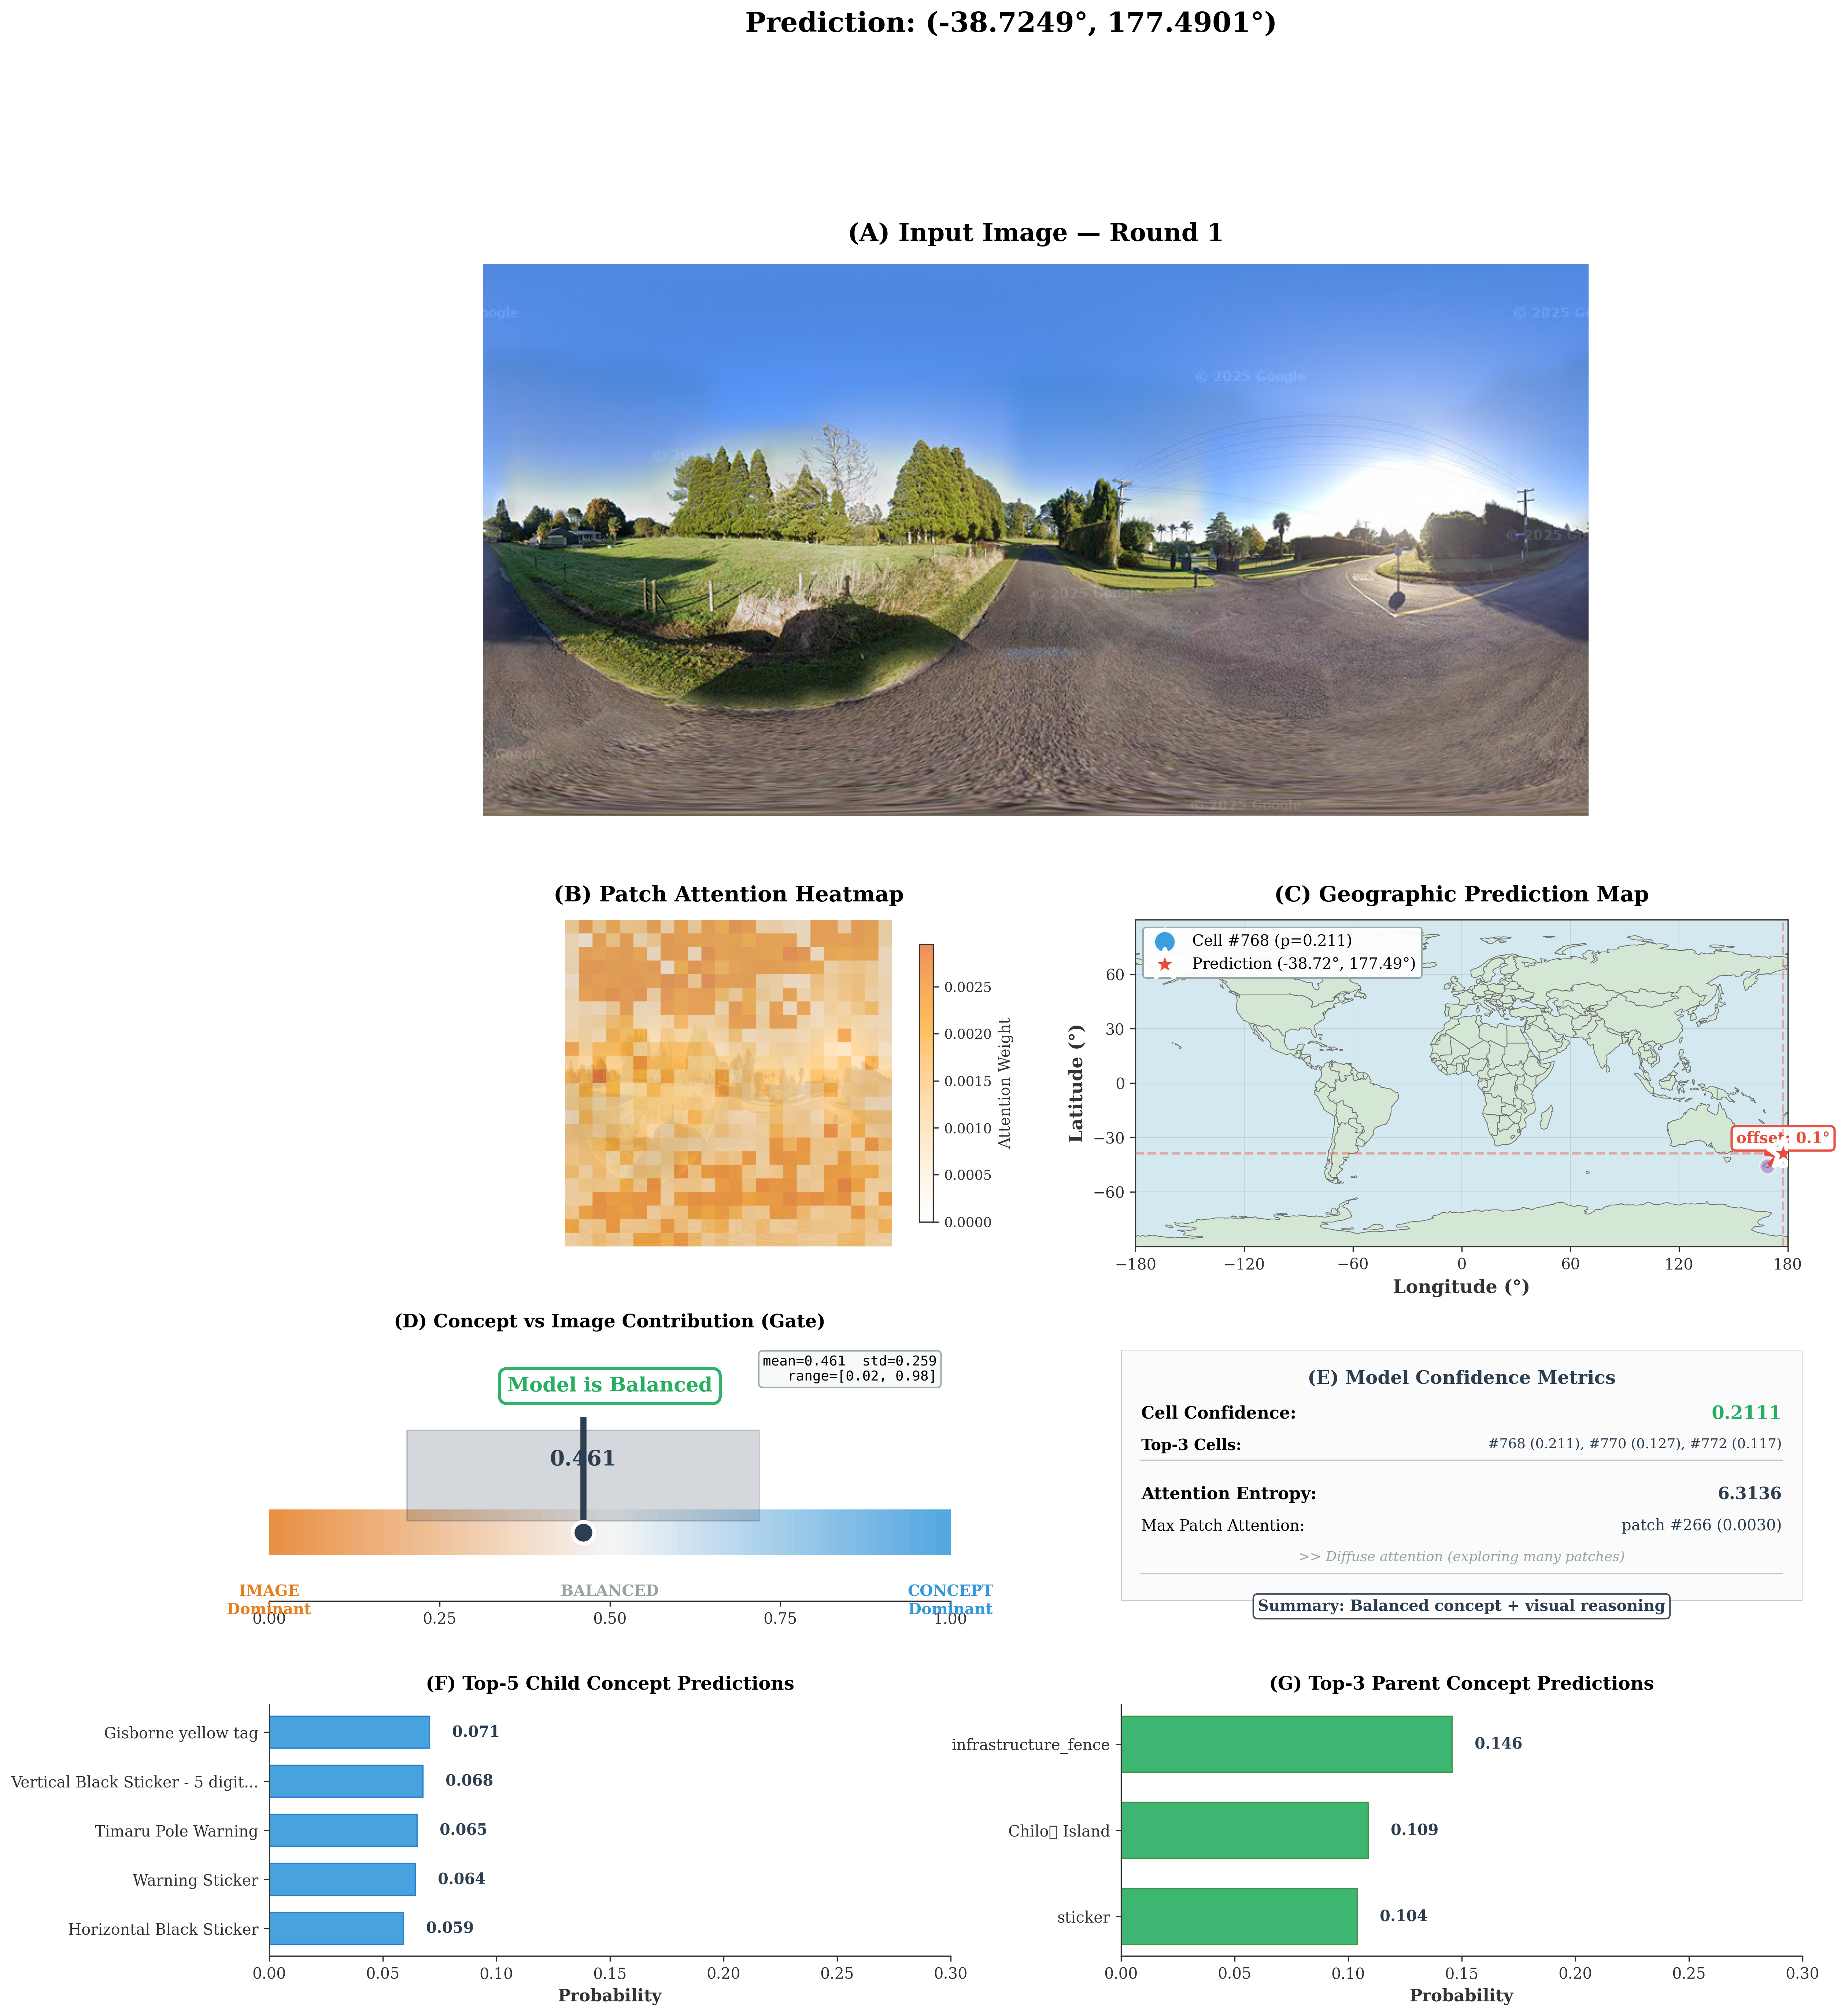
\includegraphics[width=\textwidth]{round_01_110135_concepts.png}
    \caption{Interpretability analysis for Game 1 Round 1. This example demonstrates the model attending to architectural and infrastructure features for geolocation. The patch attention heatmap reveals focus on road geometry and built structures, while concept predictions capture semantic categories relevant to the predicted region.}
    \label{fig:interpretability_example_b}
\end{figure}

\begin{figure}[h!]
    \centering
    \includegraphics[width=\textwidth]{round_09_110825_concepts.png}
    \caption{Interpretability analysis for Game 1 Round 9. The model identifies this location in West Africa through distinctive visual cues including unique vehicles and license plates, with balanced concept-spatial reasoning (gate 0.431). Top child concepts include ``Unique car'' and ``License Plates''; parent concepts indicate ``car\_meta'' and ``landscape\_savannah'' categories.}
    \label{fig:interpretability_example_a}
\end{figure}


\end{document}
